\documentclass[
	% -- opções da classe memoir --
	article,			% indica que é um artigo acadêmico
	11pt,				% tamanho da fonte
	oneside,			% para impressão apenas no recto. Oposto a twoside
	a4paper,			% tamanho do papel. 
	twocolumn,
	% -- opções da classe abntex2 --
	%chapter=TITLE,		% títulos de capítulos convertidos em letras maiúsculas
	%section=TITLE,		% títulos de seções convertidos em letras maiúsculas
	%subsection=TITLE,	% títulos de subseções convertidos em letras maiúsculas
	%subsubsection=TITLE % títulos de subsubseções convertidos em letras maiúsculas
	% -- opções do pacote babel --
	english,			% idioma adicional para hifenização
	brazil,				% o último idioma é o principal do documento
	sumario=tradicional
	]{abntex2}

\usepackage{cmap}	
\usepackage{lmodern}	
\usepackage[T1]{fontenc}	
\usepackage[utf8]{inputenc}		
\usepackage{lastpage}		
\usepackage{color}	
\usepackage{graphicx}	
\usepackage{units}
\usepackage[brazilian,hyperpageref]{backref}
\usepackage[num]{abntex2cite}
\usepackage{bold-extra}
\usepackage{eso-pic}
\usepackage{indentfirst, microtype}		
\usepackage{caption,subcaption,float, dcolumn}
\usepackage{amsfonts,amsmath,amssymb}
\usepackage{enumerate}
\usepackage{titlesec}

\usepackage{multirow}


\usepackage{algpseudocode}
\usepackage{algorithm}

\floatname{algorithm}{Algoritmo}
\renewcommand{\algorithmicrequire}{\textbf{Input:}}
\renewcommand{\algorithmicensure}{\textbf{Output:}}

\usepackage{svg}

\usepackage{listings}
\usepackage[newfloat]{minted}
% \usemintedstyle{friendly}
\citebrackets[]

\usemintedstyle{friendly}
\newenvironment{code}{\captionsetup{type=listing}}{}
\SetupFloatingEnvironment{listing}{name=Código}

\newcommand{\algorithmautorefname}{Algoritmo}
\renewcommand{\backrefpagesname}{Citado na(s) página(s):~}
\renewcommand{\backref}{}
\renewcommand*{\backrefalt}[4]{
	\ifcase #1 %
		Nenhuma citação no texto.%
	\or
		Citado na página #2.%
	\else
		Citado #1 vezes nas páginas #2.%
	\fi}%
% ---

\definecolor{blue}{rgb}{0, .226, .437}
\makeatletter
\hypersetup{
pdftitle={Circuito digital CMOS para controle do fator de qualidade de um filtro passa-banda ativo sintonizável}, 
		pdfauthor={Alef de Oliveira Santos},
    	pdfsubject={TCC2},
	    pdfcreator={LaTeX with abnTeX2},
        pdfkeywords={Fator Q. Controle digital. Métodos numéricos. RTL. Verilog.},
		colorlinks=true,       		% false: boxed links; true: colored links
    	linkcolor=blue,          	% color of internal links
    	citecolor=blue,        		% color of links to bibliography
    	filecolor=magenta,      		% color of file links
		urlcolor=blue,
		bookmarksdepth=4
}
\makeatother
\setlength{\parindent}{1.3cm}
\setlength{\parskip}{0.2cm}  
\makeindex

\renewcommand{\listalgorithmname}{Lista de algoritmos}

\titleformat{\chapter}     {\normalfont\normalsize\bfseries}{\thechapter}     				 {1em}{}
\titleformat{\section}     {\normalfont\normalsize}{\thechapter.\thesection}     			 {1em}{}
\titleformat{\subsection}  {\normalfont\normalsize}{\thechapter.\thesection.\thesubsection}  {1em}{}


\setlrmarginsandblock{1.5cm}{1.5cm}{*}
\setulmarginsandblock{1.5cm}{2.5cm}{*}
\checkandfixthelayout

\title[TCC1 - Alef de Oliveira Santos]{Circuito digital para controle do fator de qualidade de um filtro \\ passa-banda ativo sintonizável}

\subtitle{Trabalho de conclusão de curso - TCC1}

\author[Alef Santos]{\textbf{Discente:} Alef de Oliveira Santos \\ 
\textbf{Orientador:} Dr. Dean Bicudo Karolak\\
\textbf{Co-orientador}: Dr. Paulo Márcio Moreira e Silva}

\institute[UNIFEI - ICT - ECO]{Universidade federal de Itajubá - \textit{Campus} Theodomiro Carneiro Santiago \\
Instituto de Ciências Tecnológicas \\ 
Engenharia da Computação
}

\date{01 de dezembro de 2023}

\titlegraphic{\hfill
\includegraphics[width = 1cm]{lib/unifeilogo.eps}} 



\begin{document}

\AtBeginSubsection[ ]
{
\begin{frame}
    \footnotesize
    \tableofcontents
    [
        currentsection,
        currentsubsection,
        subsectionstyle=show/shaded/hide
    ]
\end{frame}
}


{
    \setbeamercolor{background canvas}{bg=secondaryColor1, fg=white}
    \setbeamercolor{normal text}{fg=black}
    \maketitle
}

\setbeamercolor{background canvas}{bg=white, fg=white}

\begin{frame}[shrink]{Sumário}
\footnotesize
    % \begin{multicols}{2}
        \setcounter{tocdepth}{3} %sumário mostrando seção e subseção apenas
        \vspace{0.3cm}
        \tableofcontents%sumário
        \vspace{0.3cm}
    % \end{multicols}
\end{frame}


\section{Introdução}


\subsection{Justificativa e contexto}

\begin{frame}{Sobre o controle do fator de qualidade neste trabalho}

\begin{itemize}
    \item O fator de qualidade ($Q$) está relacionado com a largura de banda de um filtro passa-banda;
    \item Uma vez fabricado o filtro, alterar sua banda através da modificação de parâmetros físicos é inviável;
    \item Modificar a seletividade do filtro por meio de seu fator de qualidade, que é controlado por uma corrente DC de referência, torna-se uma opção viável;
    \item Propõe-se desenvolver um circuito digital capaz de ajustar o fator de qualidade de um filtro passa-banda ativo;
    \end{itemize}
\end{frame}

\begin{frame}{\nameref{f-q-freq}}


\begin{figure}[H]
    \centering
    \caption{$Q \times$ largura de banda e sua relação com polos}
    \begin{subfigure}[H]{.49\textwidth}
        \centering
        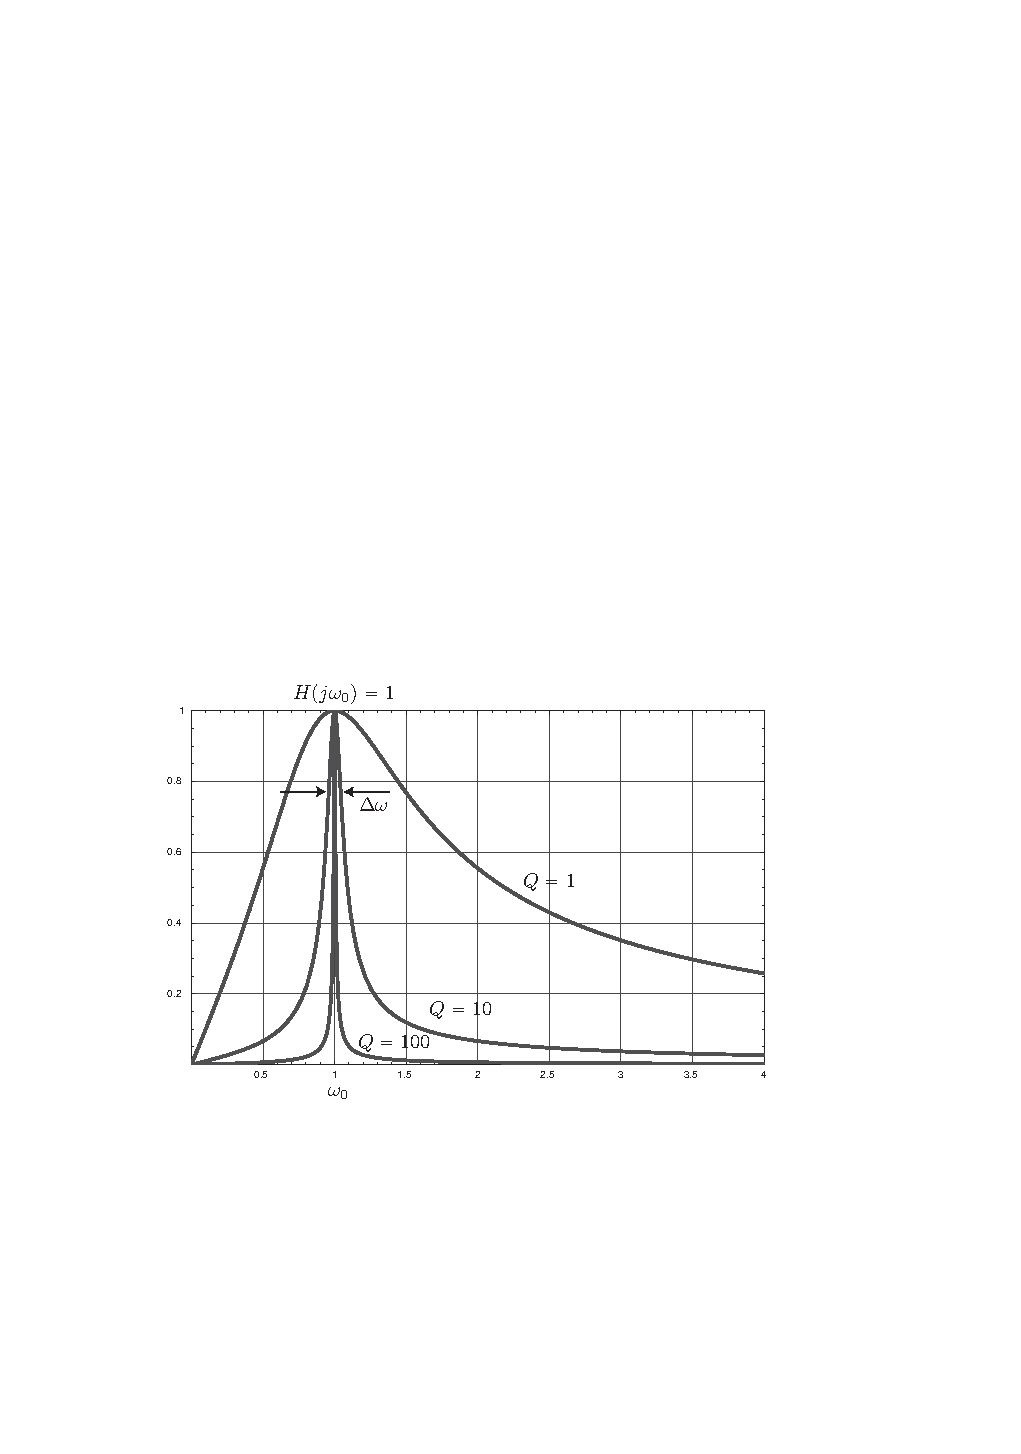
\includegraphics[width=\textwidth]{fig/q-band.pdf}
        \caption{$Q \times$ Largura de banda}
        \label{f-q-banda}
    \end{subfigure}
    \hfil
    \begin{subfigure}[H]{.49\textwidth}
        \centering
        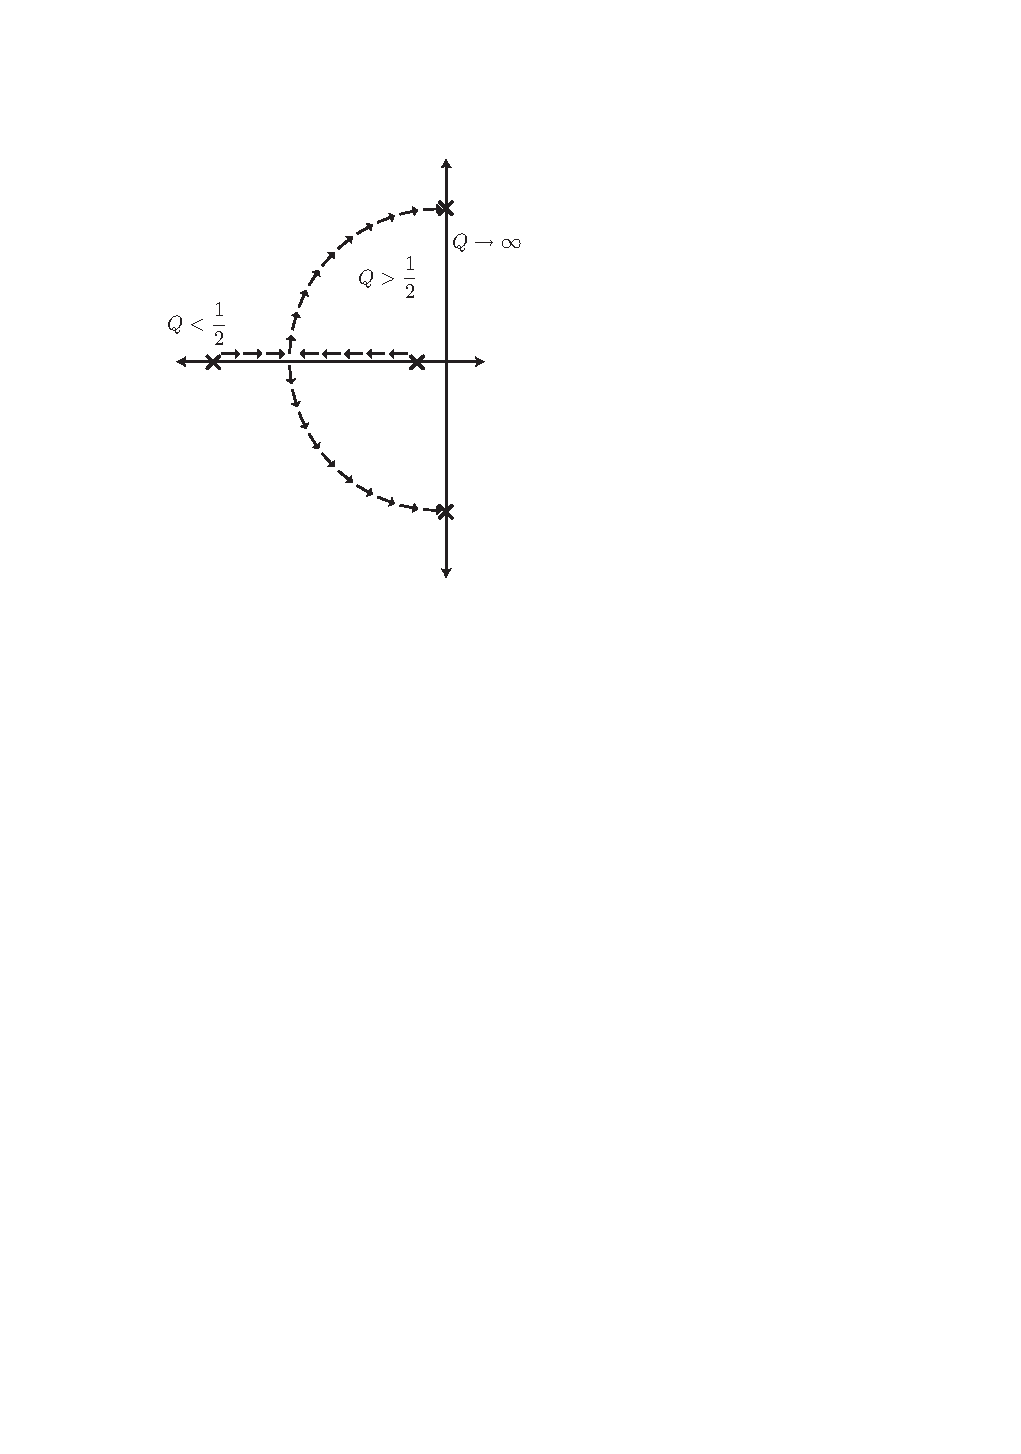
\includegraphics[width=.5\textwidth]{fig/q-poles.pdf}
        \caption{$Q$ e sua relação com polos}
        \label{f-q-polos}
    \end{subfigure}
    \label{f-q-freq}
\end{figure}

    
\end{frame}


\subsection{Requisitos do projeto}

\begin{frame}{Requisitos do projeto}

\begin{itemize}
    \item O circuito deve fazer interface adequada com o sistema pré-existente (O filtro + outras estruturas);
    \item O circuito deve controlar o $Q$ por meio de uma corrente de referência $I_{REF}$;
    \item O usuário insere um valor de $Q$ desejado ($Q_d$) e o circuito fornece um $Q$ o mais próximo possível dentro de determinada tolerância ($Q_m$), de maneira mais otimizada possível;
    \item Para controlar que o valor de $Q_m$ convirja para o valor de $Q_d$ são estudados e implementados métodos numéricos de aproximação de funções não-lineares.
\end{itemize}
    
\end{frame}

\begin{frame}

\begin{figure}[H]
    \centering
    \caption{Arquitetura simplificada do sistema completo com destaque para o filtro}
    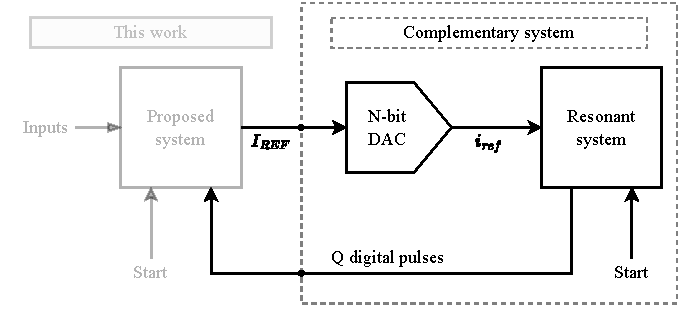
\includegraphics[width=.6\textwidth]{fig/destaque-resonant.pdf}
    \label{f-arq-destaque-resonant}
\end{figure}


    
\end{frame}


\begin{frame}[shrink]

\begin{figure}[H]
    \centering
    \caption{$Q$ e $\zeta$ no tempo}
    \begin{subfigure}[H]{.49\textwidth}
        \centering
        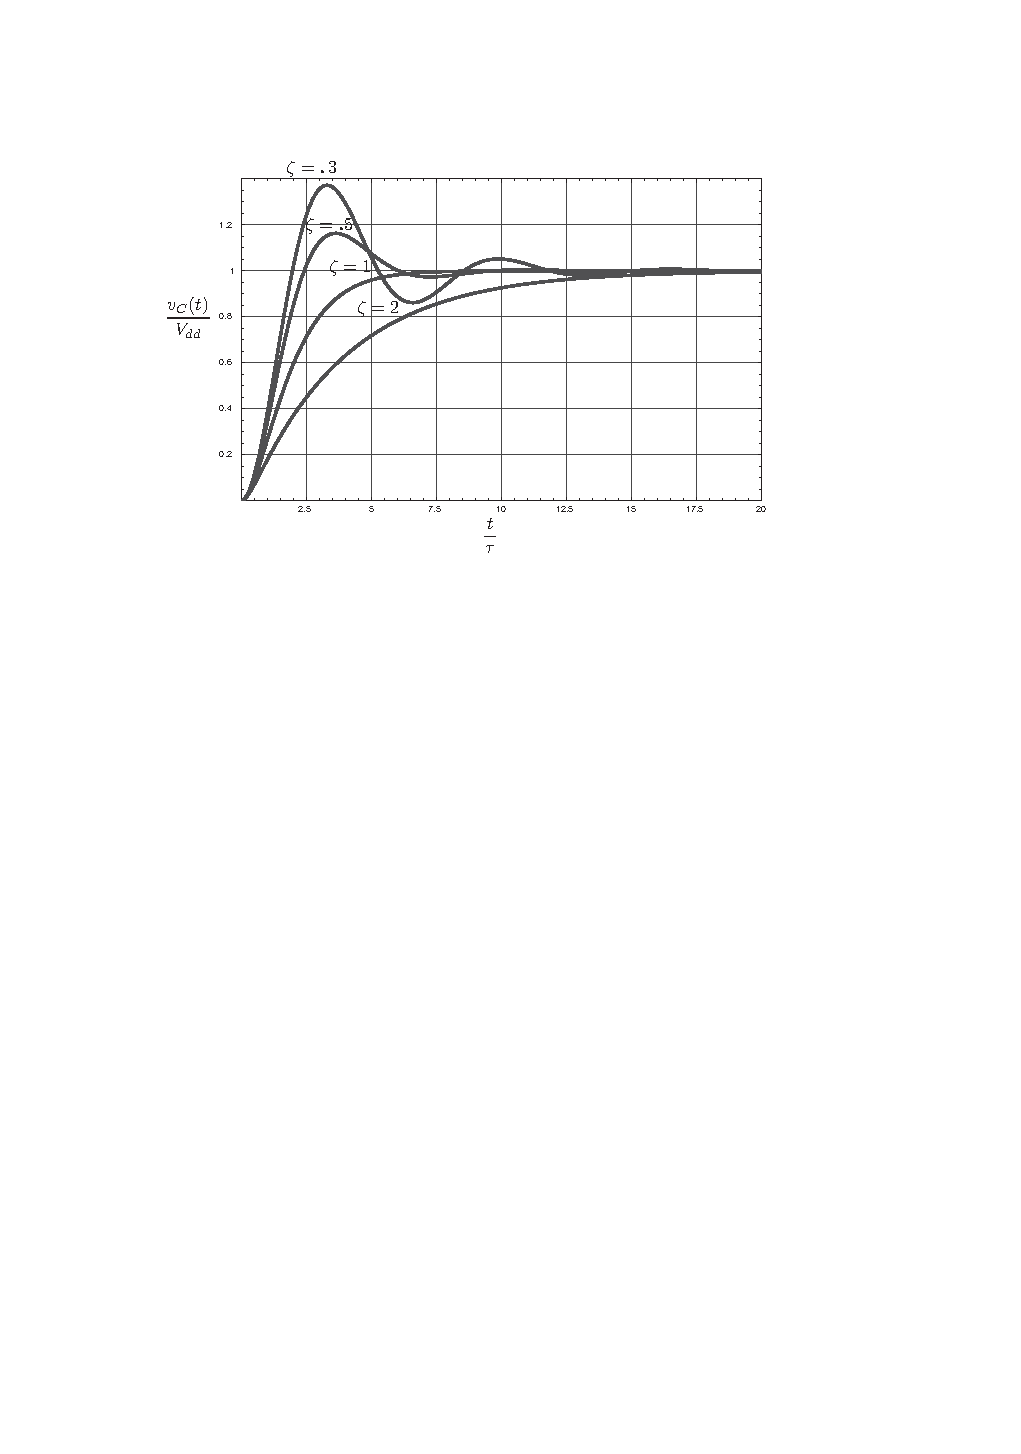
\includegraphics[width=\textwidth]{fig/q-tempo-low.pdf}
        \caption{Resposta ao degrau para diferentes valores de $\zeta$}
    \end{subfigure}
    \hfil
    \begin{subfigure}[H]{.49\textwidth}
        \centering
        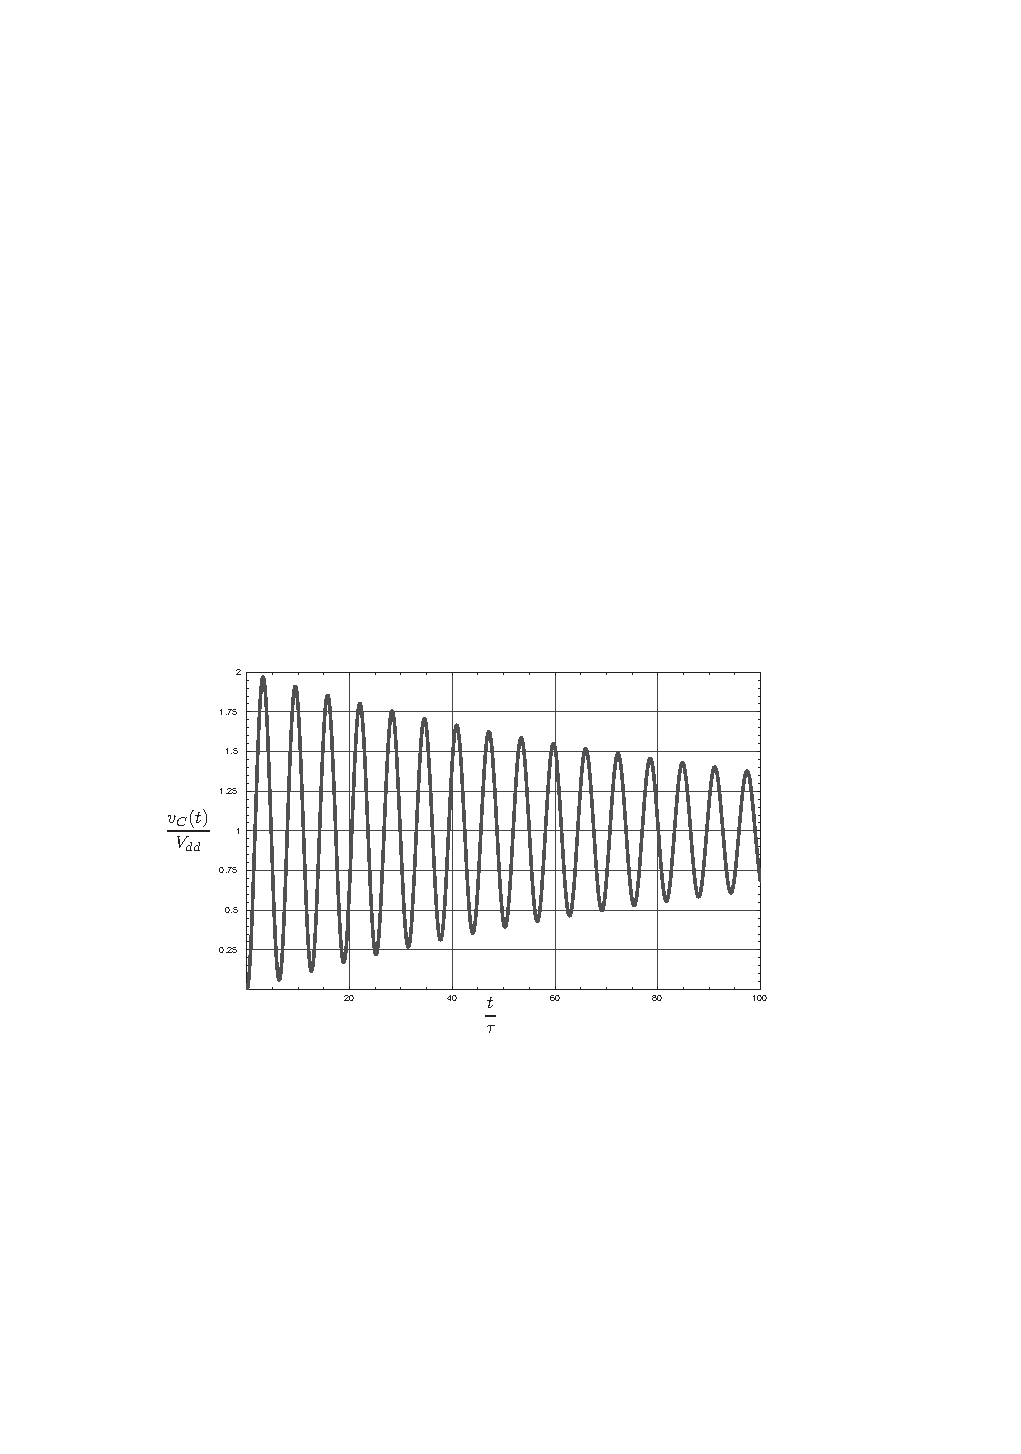
\includegraphics[width=\textwidth]{fig/q-tempo-high.pdf}
        \caption{Resposta similar à do filtro, com $\zeta = 0.01$}
    \end{subfigure}
    \label{f-q-tempo}
\end{figure}

\begin{equation}
    \zeta = \frac{1}{2Q} \quad \longleftrightarrow \quad Q = \frac{1}{2\zeta}
\end{equation}
    
\end{frame}

\begin{frame}{Curva de $Q \times I_{REF}$}

\begin{figure}[H]
    \centering
    \caption{Dados teóricos esperados e sintéticos da curva de $Q \times I_{REF}$ com a condição instabilidade}
    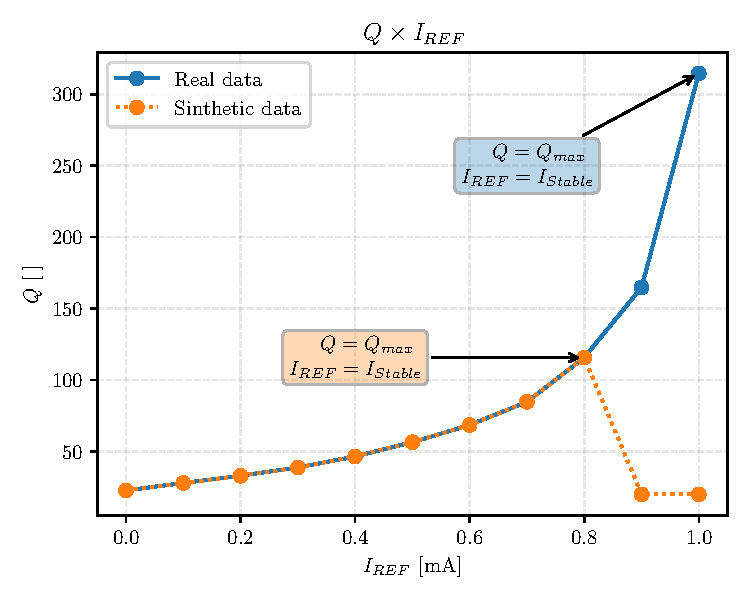
\includegraphics[width=.5\textwidth]{fig/q-iref-instability-test.pdf}
    \label{f-inst-test-inicio}
    \caption*{Fonte: o autor}
\end{figure}
    
\end{frame}

\section{Objetivos}

\begin{frame}{Objetivos para o TCC1}

Os objetivos principais deste trabalho para o TCC1 são, principalmente o fluxo de front-end, compreendido por:

\begin{enumerate}
    \item Projetar a arquitetura capaz de controlar o fator de qualidade do circuito;
    % \item Adaptar métodos numéricos e prototipá-los em alto nível
    \item Codificar os blocos do sistema projetado em Verilog;
    \item Comparar o desempenho dos métodos de controle prototipados \textit{standalone};
    \item Validar a funcionalidade blocos projetados através de \textit{testbenches} em Verilog/SystemVerilog.
\end{enumerate}

    
\end{frame}


\section{Desenvolvimento}

\subsection{Interface com o sistema completo e arquitetura simplificada}\label{sec-interface}


\begin{frame}[plain, shrink]

\begin{figure}[H]
    \centering
    \caption{Arquitetura simplificada do sistema completo}
    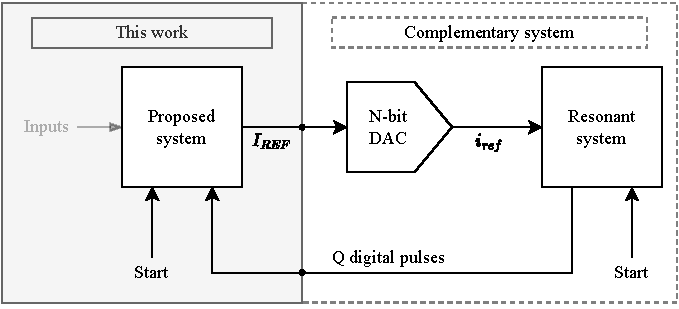
\includegraphics[width=.6\textwidth]{fig/arq-simplif.pdf}
    \label{f-arq-simplif}
\end{figure}%
\vspace*{-8pt}
\begin{table}[H]
    \centering
    \caption{Sinais, respectivos tipos e funcionalidades por bloco}
    \resizebox{\columnwidth}{!}{%
\begin{tabular}{@{}lp{3cm}lp{13cm}@{}}
\toprule
\textbf{Bloco}           & \textbf{Sinal}            & \textbf{Tipo}              & \textbf{Função referente ao bloco}                                                                    \\ \midrule
\textit{Proposed system} & Start                     & Digital {[}1 bit{]}        & Sinalizar que o oscilador enviará pulsos correspondentes ao valor de $Q$                              \\
\textit{Proposed system} & $I_{REF}$                 & Digital {[}10 bits{]}      & Enviar valor digital de corrente de referência para controlar o $Q$                                   \\
N-bit DAC                & $I_{REF}$                 & Digital {[}10 bits{]}      & Receber valor digital de corrente de referência para conversão D/A\\
N-bit DAC                & $i_{ref}$                 & Analógico                  & Equivalente analógico convertido de $I_{REF}$                                                         \\
\textit{Resonant system} & Start                     & Digital {[}1 bit{]}        & Indicar que o sistema pode injetar a corrente no oscilador LC interno                                 \\
\textit{Resonant system} & \textit{Q digital pulses} & Digital Serial {[}1 bit{]} & Valor de $Q$ medido e convertido em um trem de pulsos                                                 \\ \bottomrule
\end{tabular}%
}
    \label{tab-arq-simplif}
\end{table}

\vspace*{-12pt}
\flushright
\scriptsize
\insertframenumber~\frameofframes~\inserttotalframenumber
    
\end{frame}

% \begin{frame}{Responsabilidade de cada bloco}

% \begin{enumerate}
%     \item \textit{Proposed System}: Ajusta o $Q$
%     \item \textit{Resonant System}: Produz o $Q$
%     \item \textit{Current Control} (N-bit DAC): Realizar conversão D/A de $I_{REF}$ 
% \end{enumerate}
    
% \end{frame}


% \section{Metodologia}

\subsection{Arquitetura do sistema}

\begin{frame}[plain]

\begin{figure}[H]
    \centering
    \caption{Arquitetura desenvolvida para o sistema}
    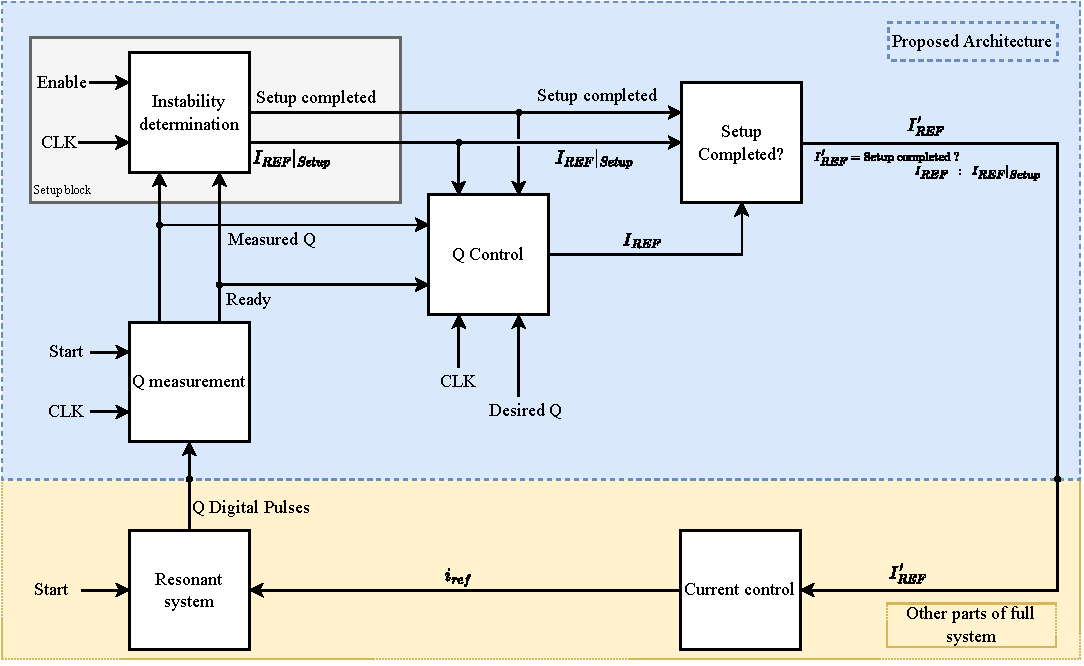
\includegraphics[width=.8\textwidth]{fig/tcc-nova-arq.pdf}
    \label{f-arq-sys}
\end{figure}

\flushright
\scriptsize
\insertframenumber~\frameofframes~\inserttotalframenumber
    
\end{frame}

\begin{frame}{Resumo da operação}

\begin{enumerate}
    \item O sistema inicializa variáveis internamente;
    \item O bloco de determinação de instabilidade retorna o maior valor admissível de corrente antes da instabilidade;
    \item O bloco de controle do $Q$ ajusta a corrente até atingir $Q_d \approx Q_m$;
    \item O sistema retém o ultimo estado para a operação normal do filtro.
\end{enumerate}
    
\end{frame}


\begin{frame}{\nameref{f-fluxograma}}
\begin{figure}[H]
    \centering
    \caption{Fluxograma de execução}
    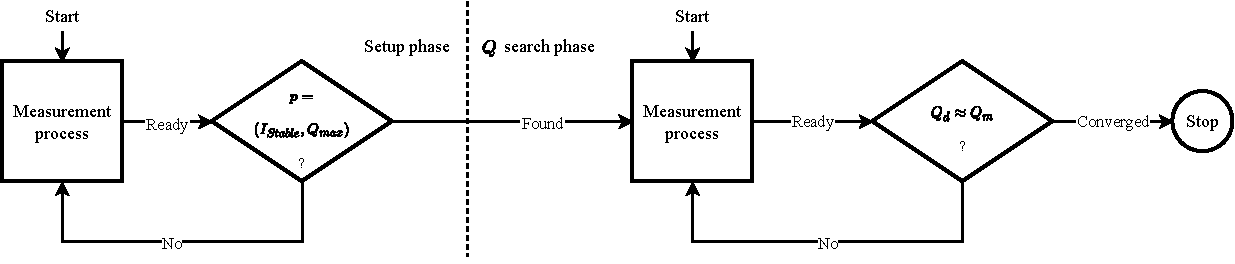
\includegraphics{fig/fluxograma.pdf}
    \label{f-fluxograma}
\end{figure}

\end{frame}

% \subsubsection{Responsabilidades por bloco}

\begin{frame}{Medição do $Q$}

\begin{figure}[H]
    \centering
    \caption{Diagrama de tempo da operação do bloco de medição.}
    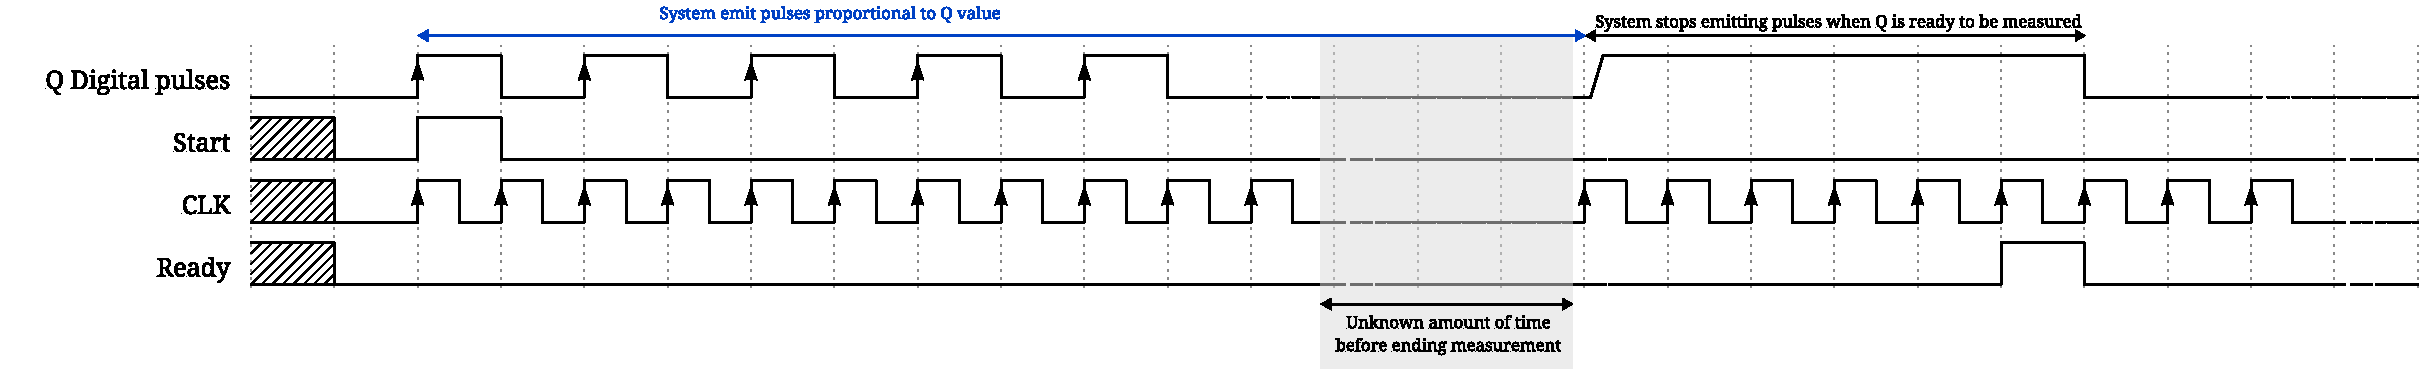
\includegraphics{fig/timing-q-measurement.pdf}
    \caption*{Fonte: o autor}
    \label{f-timing-q-measurement}
\end{figure}
    
\end{frame}

\begin{frame}{Determinação do limite de instabilidade}

\begin{figure}[H]
    \centering
    \caption{Diagrama de tempo da operação do bloco de determinação de instabilidade}
    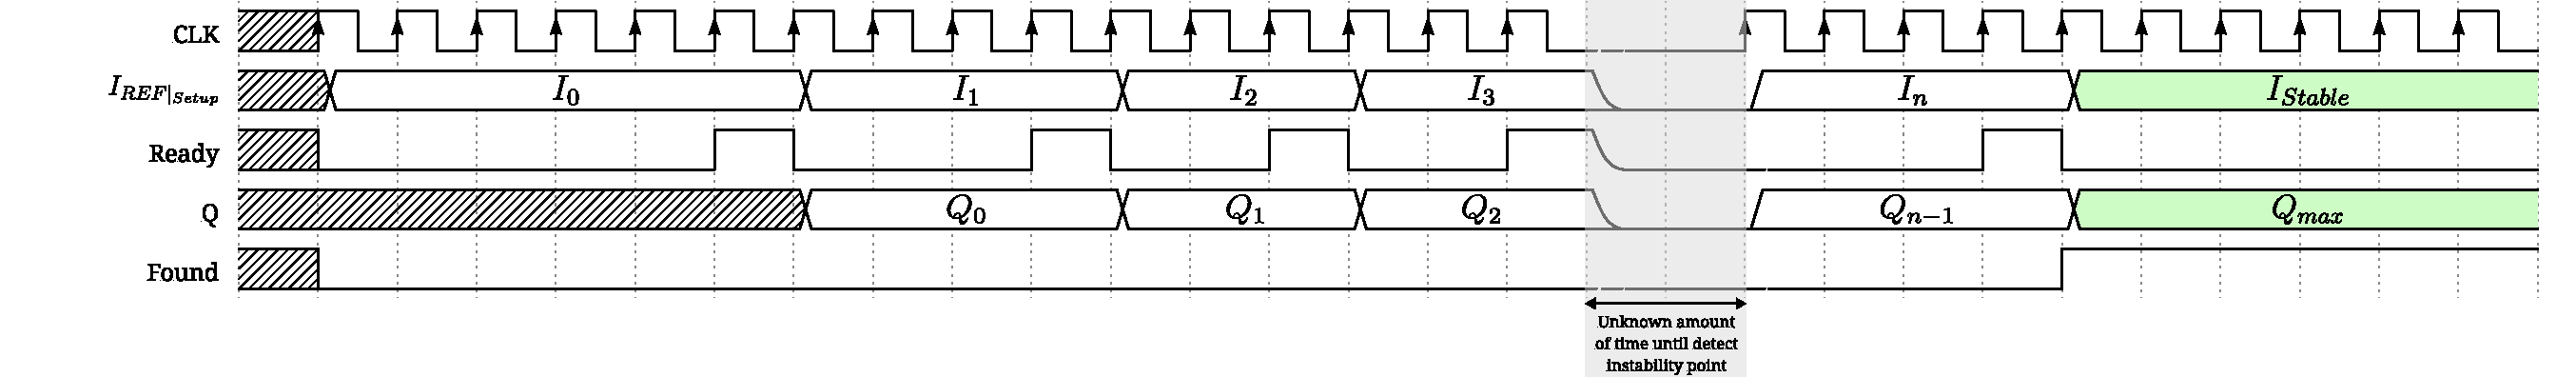
\includegraphics{fig/timing-instability-determination.pdf}
    \caption*{Fonte: o autor}
    \label{f-timing-instability-determination}
\end{figure}
    
\end{frame}

\begin{frame}{Algoritmo de detecção de instabilidade}

\begin{algorithm}[H]
    \caption{Algoritmo de determinação do ponto de instabilidade}
    \begin{algorithmic}[1]

\Require{$\Delta Q, \Delta I_{REF}$, $Q_m$}
\Ensure{$I_{Stable}$} 

\State $I_{Stable} \gets I_{MAX}$ \Comment{$I_{MAX} =$ 1mA}
\State Found $\gets$ \textbf{False}

\While{not Found}
    
    \State $Q_i \gets Q_m(I_{Stable})$\Comment{Medição}
    \State $I_{Stable} \gets I_{Stable}  - \Delta I_{REF}$
    \State $Q_{i+1} \gets Q_m(I_{Stable})$\Comment{Nova medição}
    \If{$\left(Q_{i+1} - Q_i \geq \Delta Q\right)$}
        \State Found $\gets$ \textbf{True}
    \EndIf
\EndWhile
\State \textbf{return $I_{Stable}$}
\end{algorithmic}
\end{algorithm}
    
\end{frame}

\begin{frame}{Seleção de correntes}

\begin{figure}[H]
    \centering
    \caption{Diagrama de tempo da operação do bloco de seleção de corrente}
    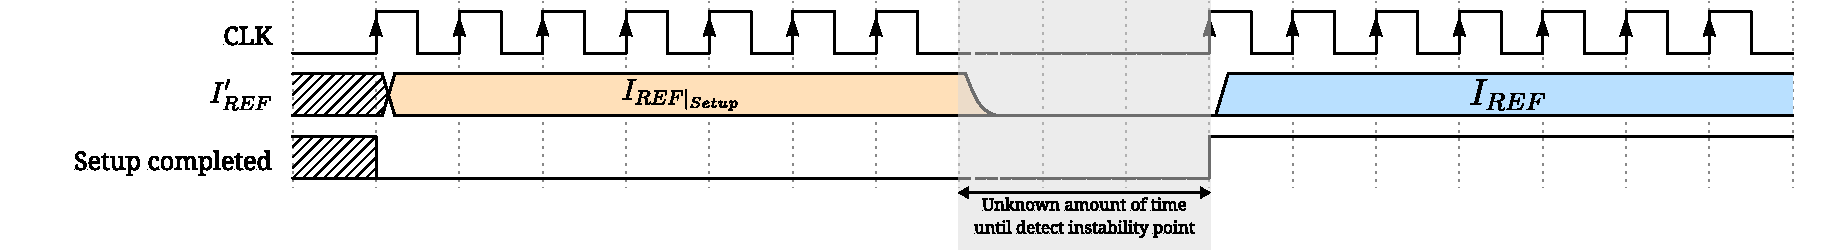
\includegraphics{fig/timing-iref-selection.pdf}
    \caption*{Fonte: o autor}
    \label{f-timing-iref-selection}
\end{figure}
    
\end{frame}

\begin{frame}{Representação do bloco de seleção de correntes}

\begin{figure}[H]
    \centering
    \caption{Representação do bloco intertravamento ou seleção de correntes}
    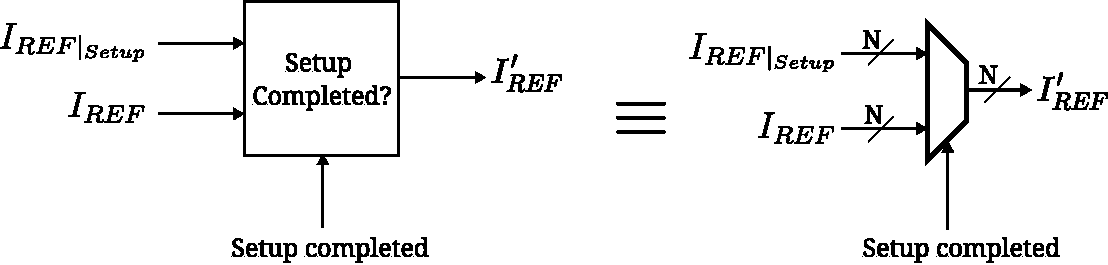
\includegraphics[width=.9\textwidth]{fig/setup-completed-equiv.pdf}
    \label{f-bloco-setup-completed}
\end{figure}
    
\end{frame}

\begin{frame}{Controle do $Q$}
\begin{figure}[H]
    \centering
    \caption{Diagrama de tempo da operação do bloco de controle do $Q$.}
    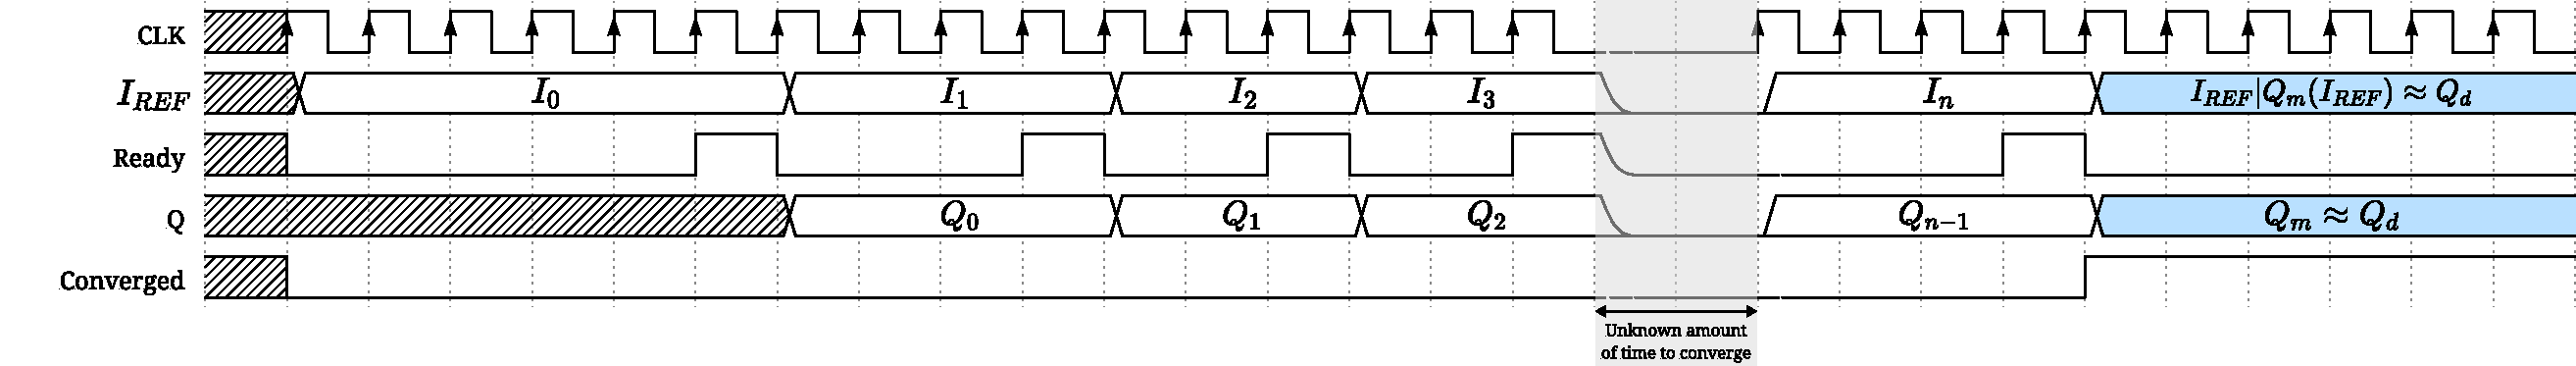
\includegraphics{fig/timing-q-control.pdf}
    \caption*{Fonte: o autor}
    \label{f-timing-q-control}
\end{figure}
    
\end{frame}


% \subsection{Adaptação de métodos numéricos para busca de valores}\label{sec-adapt-metodos}

\begin{frame}[shrink]{\nameref{alg-bi}}
\scriptsize
\begin{algorithm}[H]
    \scriptsize
    \caption{Método adaptado da bisseção}
    \begin{algorithmic}[1]

\Require TOL, $Q_{d}$, $Q_{m}$, $I_{Stable}$
\Ensure $I_{REF} \; | \; \varepsilon \leq$ TOL

\State $a \gets 0$
\State $b \gets I_{Stable}$
\State Converged $\gets$ \textbf{False}
 
\While{not Converged}

    \State $c \gets \frac{a+b}{2}$
% \Comment{$I_{REF}$ is updated to "c"\; value}

    \State $I_{REF} \gets c$ 

    \State $Q_{m} \gets Q_{m}\left(I_{REF}\right)$ \Comment{Realiza-se uma medição do $Q$ com o novo valor de $I_{REF}$}

    \State $\varepsilon \gets Q_m - Q_d $

    \If{$\varepsilon \leq $ TOL} Converged $\gets$ \textbf{True} 
        \Else
            \If{$\varepsilon > 0$}
                \State $a \gets c$
            \EndIf
            \If{$\varepsilon < 0$}
                \State $b \gets c$
            \EndIf
    \EndIf

\EndWhile
\end{algorithmic}
    \label{alg-bi}
\end{algorithm}
\end{frame}

\begin{frame}[shrink]{\nameref{alg-sec}}
\scriptsize
\begin{algorithm}[H]
    \scriptsize
    \caption{Método adaptado das secantes}
    \begin{algorithmic}[1]

\Require TOL, $Q_{d}$, $Q_{m}$, $I_{Stable}$
\Ensure $I_{REF} \; | \; \varepsilon \leq$ TOL

\State $a \gets 0$
\State $b \gets I_{Stable}$
\State Converged $\gets$ \textbf{False}

\While{not Converged} \\

    \State slope $ \gets \dfrac{Q_m(b) - Q_m(a)}{b-a}$ \Comment{$Q_m(a), Q_m(b)$ são novas medições} \\
    \State $c \gets b - \dfrac{Q_m(b) - Q_d}{\text{slope}}$
    \State $I_{REF} \gets c$

    \State $Q_{m} \gets Q_{m}\left(I_{REF}\right)$  \Comment{Medição do $Q$ com o novo valor de $I_{REF}$}

    \State $\varepsilon \gets \left|Q_m - Q_d \right|$

    \If{$\varepsilon \leq $ TOL} Converged $\gets$ \textbf{True} 
        \Else
            \State $a \gets b$
            \State $b \gets c$
    \EndIf

\EndWhile
\end{algorithmic}
    \label{alg-sec}
\end{algorithm}
\end{frame}

\begin{frame}{Método das secantes com seleção de intervalo}

\begin{itemize}
    \item O desempenho do método das secantes varia drasticamente com a seleção do intervalo inicial de busca.
    \item Há duas regiões com comportamentos distintos que aceleram a convergência se detectados previamente.
\end{itemize}
\end{frame}

\begin{frame}{Representação gráfica da seleção de intervalo}
    


\begin{figure}[H]
    \centering
    \caption{$Q \times I_{REF}$ com destaque para as regiões linear e não linear}
    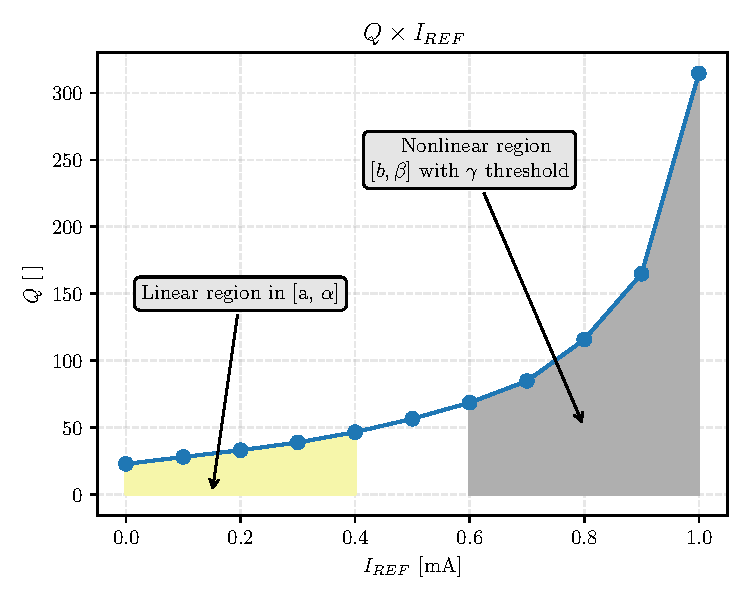
\includegraphics[width = .5\textwidth]{fig/q-iref-regions.pdf}
    \label{f-q-iref-regioes}
\end{figure}
    
\end{frame}

\begin{frame}[shrink]{\nameref{alg-mod-sec}}
\scriptsize
\begin{algorithm}[H]
    \scriptsize
    \caption{Método adaptado das secantes com seleção de intervalo desenvolvido}
    \begin{algorithmic}[1]

\Require TOL, $Q_{d}$, $Q_{m}$, $I_{Stable}$
\Ensure $I_{REF} \; | \; \varepsilon \leq$ TOL

\State Converged $\gets$ \textbf{False}
\State $Q_{max} \gets Q_m(I_{Stable})$
\If{$Q_d > \gamma \cdot Q_{max}$} \Comment{Seleção na região linear}
    \State $a \gets \alpha \cdot I_{Stable}$
    \State $b \gets I_{Stable}$
    \Else \Comment{Seleção na região não-linear}
        \State $a \gets 0$
        \State $b \gets \beta \cdot I_{Stable}$
\EndIf


\While{not Converged}  \\
    \State slope $ \gets \dfrac{Q_m(b) - Q_m(a)}{b-a}$
    \Comment{$Q_m(a), Q_m(b)$ são novas medições} \\
    \State $c \gets b - \dfrac{Q_m(b) - Q_d}{\text{slope}}$
    \State $I_{REF} \gets c$

    \State $Q_{m} \gets Q_{m}\left(I_{REF}\right)$  \Comment{Medição do $Q$ com o novo valor de $I_{REF}$}

    \State $\varepsilon \gets \left|Q_m - Q_d \right|$

    \If{$\varepsilon \leq $ TOL} Converged $\gets$ \textbf{True} 
        \Else
            \State $a \gets b$
            \State $b \gets c$
    \EndIf

\EndWhile
\end{algorithmic}
    \label{alg-mod-sec}
\end{algorithm}
\end{frame}

\section{Resultados e análise}

\subsection{Bloco de determinação da instabilidade}

\begin{frame}

\begin{figure}[H]
    \centering
    \caption{Destaque do DUT: \textit{Instability determination}}
    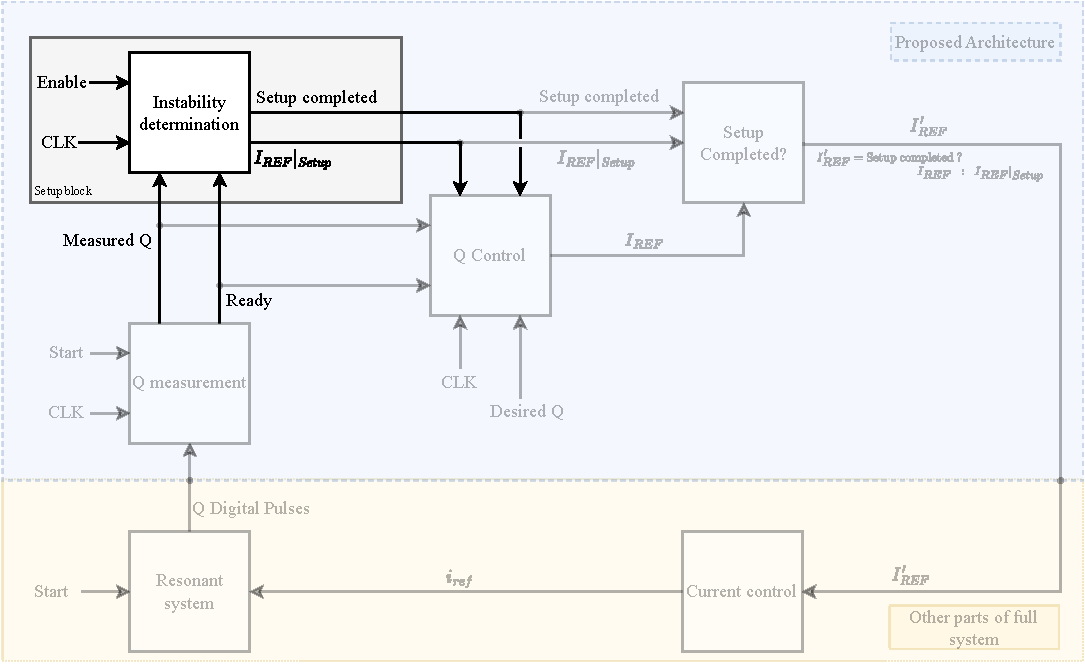
\includegraphics[width=.6\textwidth]{fig/destaque-inst-detect.pdf}
    \label{f-destaque-inst-detext}
    \caption*{Fonte: o autor}
\end{figure}
    
\end{frame}

\begin{frame}{Dados usados}

\begin{figure}[H]
    \centering
    \caption{Dados teóricos e sintéticos utilizados para o teste de determinação de instabilidade}
    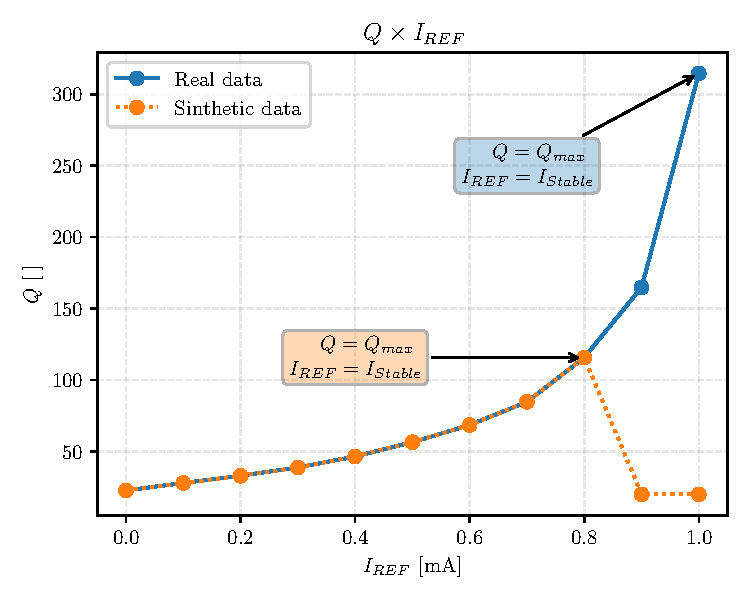
\includegraphics[width=.5\textwidth]{fig/q-iref-instability-test.pdf}
    \label{f-inst-test}
    \caption*{Fonte: o autor}
\end{figure}
    
\end{frame}

\begin{frame}{Especificações e parâmetros}

\begin{table}[H]
    \centering
    \caption{Parâmetros passados ao algoritmo de determinação de instabilidade}
    \resizebox{\textwidth}{!}{%
\begin{tabular}{lll}
\hline
\textbf{Parâmetro}& \textbf{Valor} & \textbf{Descrição}                            \\ \hline
$\Delta Q$                              & 50 [ ]                             & Variação de $Q$ considerada suficiente para sair da região instável \\
$\Delta I_{REF}$                        & 10 [bits]                          & Valor de decremento da corrente de configuração                     \\
$p = (I_{Stable}, Q_{max})$            & (850 [bits], 113 [ ])              & Ponto (definido) de estabilidade                                    \\
MAX\_ITER                               & 50                                 & Numero máximo de iterações. (neste caso são ciclos de clock)        \\ \hline
\end{tabular}%
}
    \label{tab-spec-inst}
     \caption*{Fonte: o autor}
\end{table}
    
\end{frame}

\begin{frame}{Resultados da busca}

\begin{table}[H]
    \centering
    \caption{Resultados da busca por ponto máximo de estabilidade.}
    \begin{tabular}{rrrr}
\toprule
 Time &  $I_{REF}$ [bits] &  $Q_m$ &  $I_{REF}$ [mA] \\
\midrule
    2 &   1013 &   23 &    0.989258 \\
    7 &    993 &   23 &    0.969727 \\
   12 &    963 &   23 &    0.940430 \\
   17 &    943 &   23 &    0.920898 \\
   22 &    913 &   23 &    0.891602 \\
   27 &    893 &   23 &    0.872070 \\
   32 &    863 &   23 &    0.842773 \\
   36 &    843 &   113 &   0.823242 \\
\bottomrule
\end{tabular}

    \label{tab-teste-inst}
     \caption*{Fonte: o autor}
\end{table}
    
\end{frame}

\begin{frame}{Comentários sobre a busca do ponto de instabilidade}

\begin{itemize}
    \item Da Tabela \autoref{tab-teste-inst} verifica-se que o ponto de estabilidade é determinado como 843 enquanto o esperado é 850 após 36 ciclos de \textit{clock}. 

    \item Os parâmetros de $\Delta I_{REF}, \Delta Q$ foram ajustados priorizando a proximidade com o ponto definido (850). 
    
    \item Pode-se priorizar a rapidez da busca em troca de obter um $Q_{max}$ menor ajustando os parâmetros.
\end{itemize}
    
\end{frame}

\subsection{Bloco de controle do $Q$}

\begin{frame}

\begin{figure}[H]
    \centering
    \caption{Destaque do DUT: $Q$ \textit{Control}}
    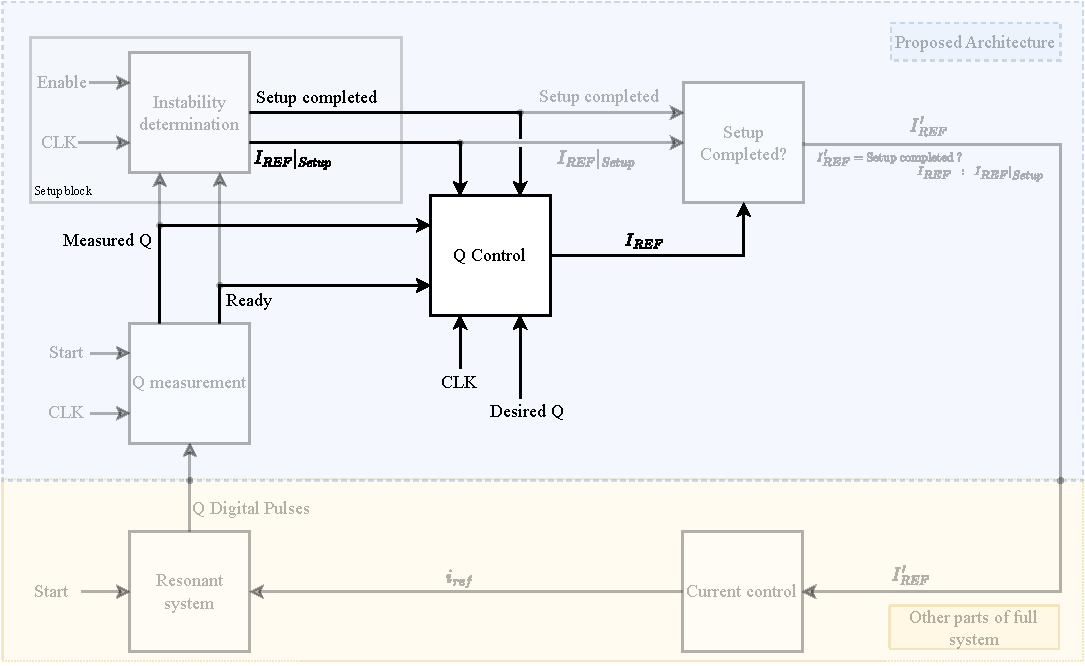
\includegraphics[width=.6\textwidth]{fig/destaque-q-control.pdf}
    \label{f-destaque-q-control}
    \caption*{Fonte: o autor}
\end{figure}
    
\end{frame}

\subsubsection{Algoritmos em alto nível}

\begin{frame}{Especificações da busca por valor único -- Cenário padrão}
    \begin{table}[H]
        \centering
        \caption{Especificações do teste de busca por valor único}
        \begin{tabular}{@{}lll@{}}
\toprule
\textbf{Parâmetro} & \textbf{Valor} & \textbf{Descrição}                   \\ \midrule
$a$                & 0.0            & Limite inferior inicial de $I_{REF}$ \\
$b$                & 1.0            & Limite superior inicial de $I_{REF}$ \\
TOL                & $\pm 30$       & Tolerância ou erro máximo admissível \\
$Q_d$              & 110            & Valor de Q desejado                  \\
MAX\_ITER           & 32             & Numero máximo de iterações.          \\ \bottomrule
\end{tabular}
        \label{tab-spec-single}
        \caption*{Fonte: o autor}
    \end{table}
    
\end{frame}

\begin{frame}{Resultados dos métodos}

\begin{figure}[H]
    \centering
    \caption{Pontos obtidos por iteração e curva $Q \times I_{REF}$ dos métodos de busca em alto nível}
    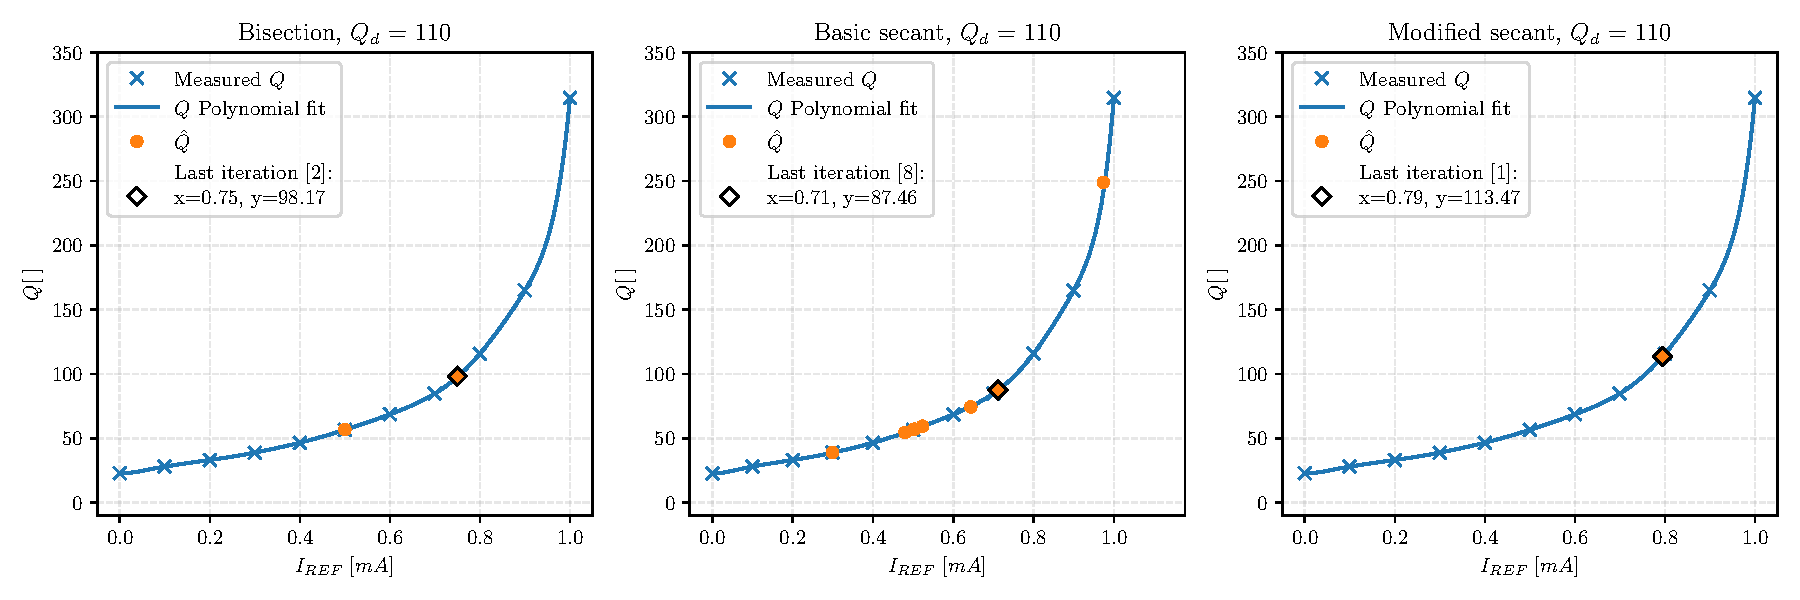
\includegraphics{fig/res-methods-single.pdf}
    \caption*{Fonte: o autor}
    \label{f-res-single}
\end{figure}
    
\end{frame}

\begin{frame}[standout]

Busca em sweep no cenário realista
    
\end{frame}

\begin{frame}{Especificações da busca em \textit{sweep} no cenário realista}
    
\begin{table}[H]
    \centering
    \caption{Especificações do teste de busca em \textit{sweep}}
    \begin{tabular}{@{}lll@{}}
\toprule
\textbf{Parâmetro} & \textbf{Valor} & \textbf{Descrição}                   \\ \midrule
$a$                & 0.0 [mA]            & Limite inferior inicial de $I_{REF}$ \\
$b$                & 1.0 [mA]            & Limite superior inicial de $I_{REF}$ \\
TOL                & $\pm 30$       & Tolerância ou erro máximo admissível \\
$Q_d$              & 30 até 300 com passo de 20           & Valor de Q desejado                  \\
MAX\_ITER           & 32             & Numero máximo de iterações.          \\ \bottomrule
\end{tabular}
     \caption*{Fonte: o autor}
    \label{tab-spec-sweep}
\end{table}

\end{frame}

\begin{frame}{\nameref{fig-itc-q-trend}}

\begin{figure}[H]
    \centering
    \caption{Número de iterações para convergência e valor desejado de $Q$ com alta tolerância}
    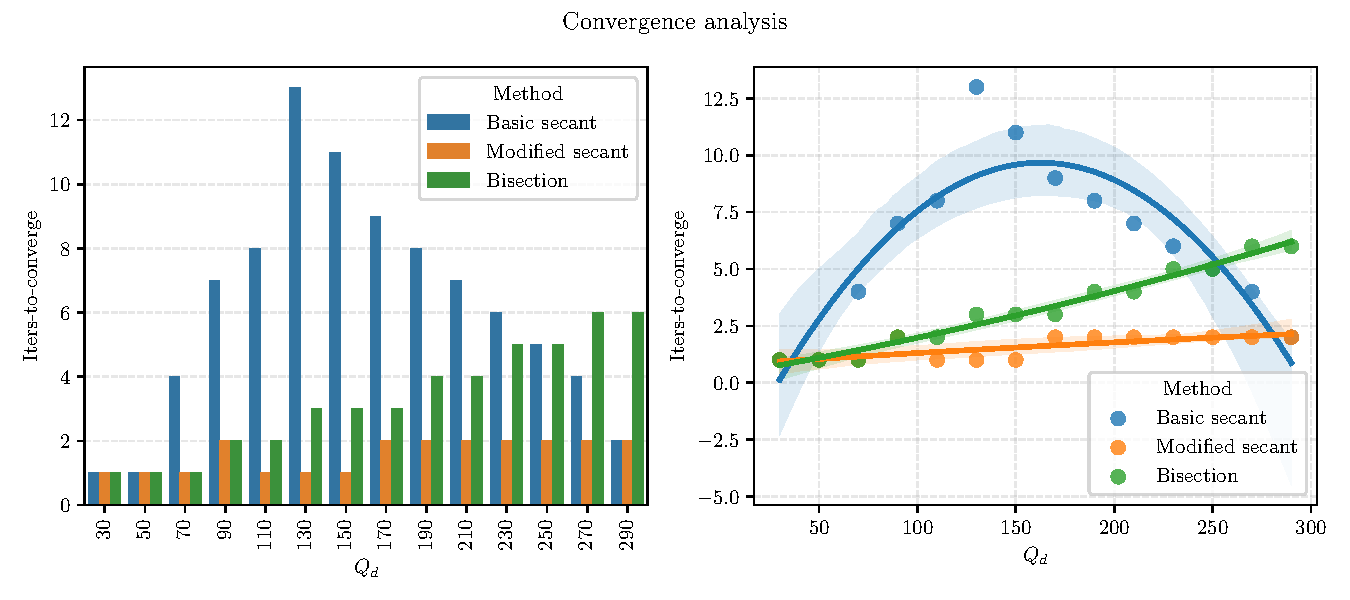
\includegraphics[width=.8\textwidth]{fig/conv-analysis-no-drop.pdf}
     \caption*{Fonte: o autor}
    \label{fig-itc-q-trend}
\end{figure}
    
\end{frame}

\begin{frame}{Estatísticas da busca em \textit{sweep}}

\begin{table}[H]
    \centering
    \caption{Tabela com mínimo, máximo, média, desvio e variância de ITC por método}
        \begin{tabular}{lrrrrr}
\toprule
{} &              Min &              Max &              Mean &               STD &               VAR \\
{} & ITC & ITC & ITC & ITC & ITC \\
\midrule
Basic secant    &                 1 &                13 &          6.142857 &          3.591810 &         12.901099 \\
Bisection       &                 1 &                 6 &          3.285714 &          1.772811 &          3.142857 \\
Modified secant &                 1 &                 2 &          1.571429 &          0.513553 &          0.263736 \\
\bottomrule
\end{tabular}

    \caption*{Fonte: o autor}
    \label{tab-stats-sweep}
\end{table}
    
\end{frame}


\begin{frame}[standout]

Busca em sweep no cenário sintético (baixa tolerância), TOL $ = \pm 1$
    
\end{frame}



\begin{frame}{Resultados dos métodos no cenário sintético}
\begin{figure}[H]
    \centering
    \caption{Número de iterações para convergência e valor desejado de $Q$ com baixa tolerância}
    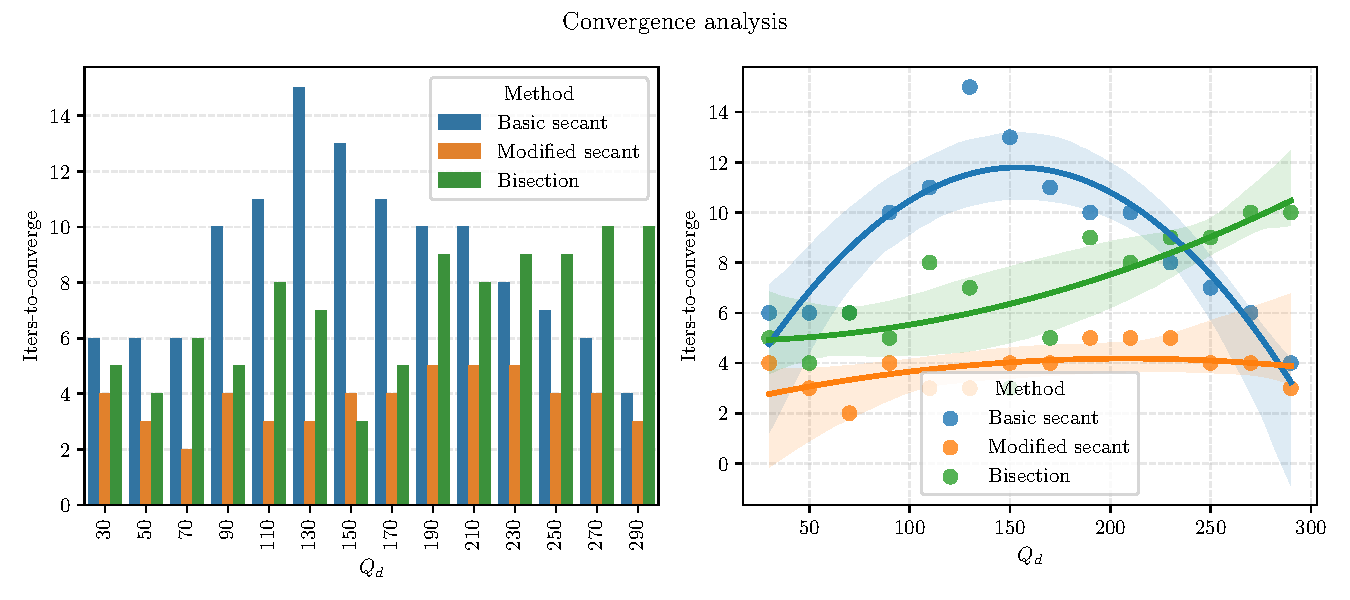
\includegraphics[width=.8\textwidth]{fig/conv-analysis-no-drop-low-tol.pdf}
     \caption*{Fonte: o autor}
    \label{fig-itc-q-trend-low-tol}
\end{figure}

    
\end{frame}

\begin{frame}{Estatísticas da busca em \textit{sweep}}

\begin{table}[H]
    \centering
    \caption{Tabela com mínimo, máximo, média, desvio e variância de ITC por método}
        \begin{tabular}{lrrrrr}
\toprule
{} &              Min &              Max &              Mean &               std &               var \\
{} & ITC & ITC & ITC & ITC & ITC \\
\midrule
Basic secant    &                 4 &                15 &          8.785714 &          3.142233 &          9.873626 \\
Bisection       &                 3 &                10 &          7.000000 &          2.320477 &          5.384615 \\
Modified secant &                 2 &                 5 &          3.785714 &          0.892582 &          0.796703 \\
\bottomrule
\end{tabular}

 \caption*{Fonte: o autor}
    \label{tab-stats-sweep-low-tol}
\end{table}
    
\end{frame}

\subsubsection{Algoritmos em HDL}

\begin{frame}[standout]

Resultados do método da bisseção em HDL, TOL $\pm 1$
    
\end{frame}

\begin{frame}{\autoref{tab-res-single-bisect}}


\begin{multicols}{2}

\begin{table}[H]
    \centering
    \caption{Pontos obtidos por iteração no método da bisseção}
        \begin{tabular}{ccc}
\toprule
$I_{REF}$ [bits] & $I_{REF} \; [mA]$ & $Q_m$ \\
\midrule
                511 &          0.499511 &    56 \\
                767 &          0.749756 &    97 \\
                895 &          0.874878 &   151 \\
                831 &          0.812317 &   121 \\
                799 &          0.781036 &   108 \\
                815 &          0.796676 &   114 \\
                807 &          0.788856 &   111 \\
                803 &          0.784946 &   110 \\
\bottomrule
\end{tabular}

        \caption*{Fonte: o autor}
    \label{tab-res-single-bisect}
\end{table}
\vfill
\begin{figure}[H]
    \centering
    \caption{Gráfico dos pontos obtidos por iteração no método da bisseção}
    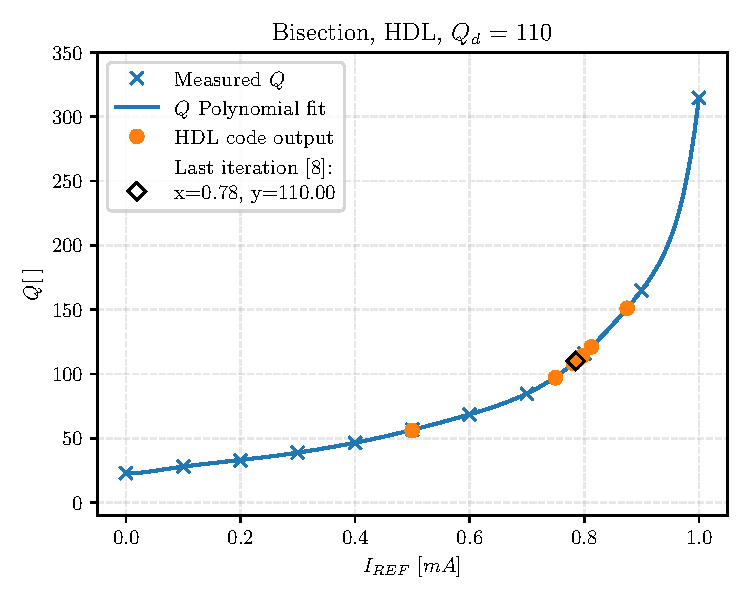
\includegraphics[width=.4\textwidth]{fig/res-bisect-single-hdl.pdf}
     \caption*{Fonte: o autor}
    \label{f-res-single-bisect}
\end{figure}
\end{multicols}
    
\end{frame}

\begin{frame}{Comparativo entre implementações de baixo e alto nível}

\begin{figure}[H]
    \centering
    \caption{Número de iterações para convergência \textit{versus} $Q_d$ do método da bisseção em de HDL \textit{versus} PL}
    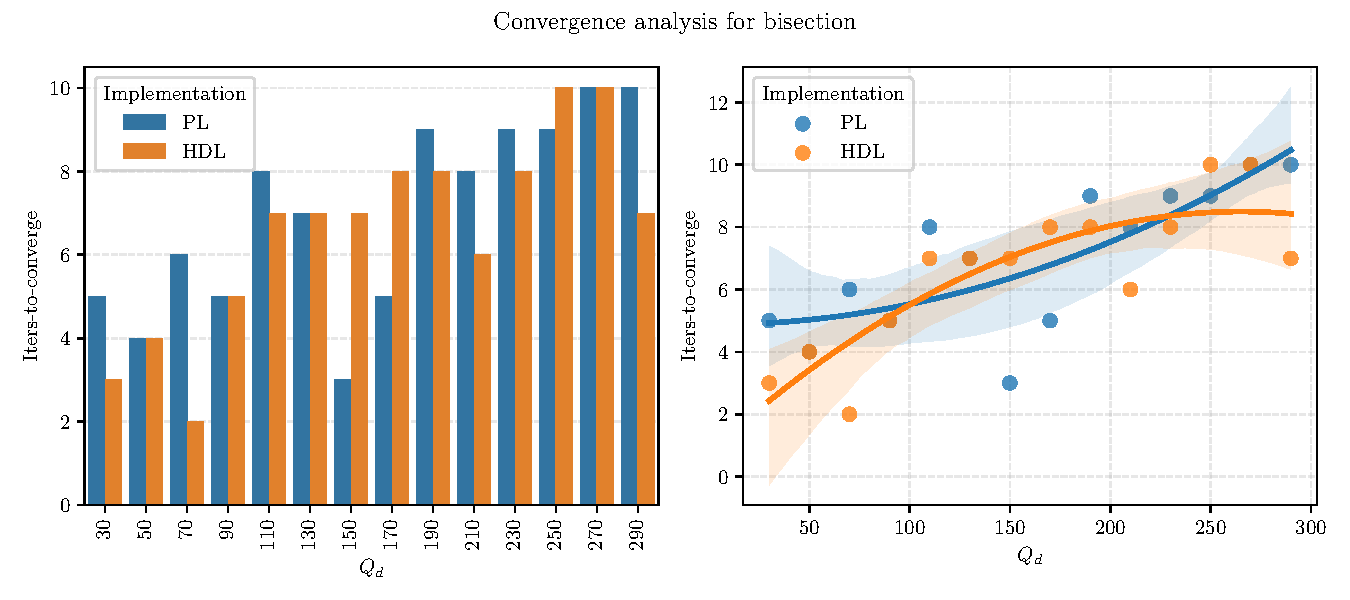
\includegraphics[width=.8\textwidth]{fig/conv-analysis-no-drop-bisect.pdf}
     \caption*{Fonte: o autor}
    \label{f-itc-q-trend-low-tol-bisect}
\end{figure}
    
\end{frame}

\begin{frame}{Estatísticas das implementações}

\begin{table}[H]
    \centering
    \caption{Tabela com mínimo, máximo, média, desvio e variância de ITC por implementação}
        \begin{tabular}{lrrrrr}
\toprule
{} &              amin &              amax &              mean &               std &               var \\
{} & Iters-to-converge & Iters-to-converge & Iters-to-converge & Iters-to-converge & Iters-to-converge \\
Implementation &                   &                   &                   &                   &                   \\
\midrule
HDL            &                 2 &                10 &          6.571429 &          2.376626 &          5.648352 \\
PL             &                 3 &                10 &          7.000000 &          2.320477 &          5.384615 \\
\bottomrule
\end{tabular}

     \caption*{Fonte: o autor}
    \label{tab-stats-low-tol-bisect}
\end{table}
    
\end{frame}

\begin{frame}{\nameref{f-sweep-bisect}}

\begin{figure}[H]
    \centering
    \caption{Busca em sweep dos valores de $Q_d$ no método da bisseção}
    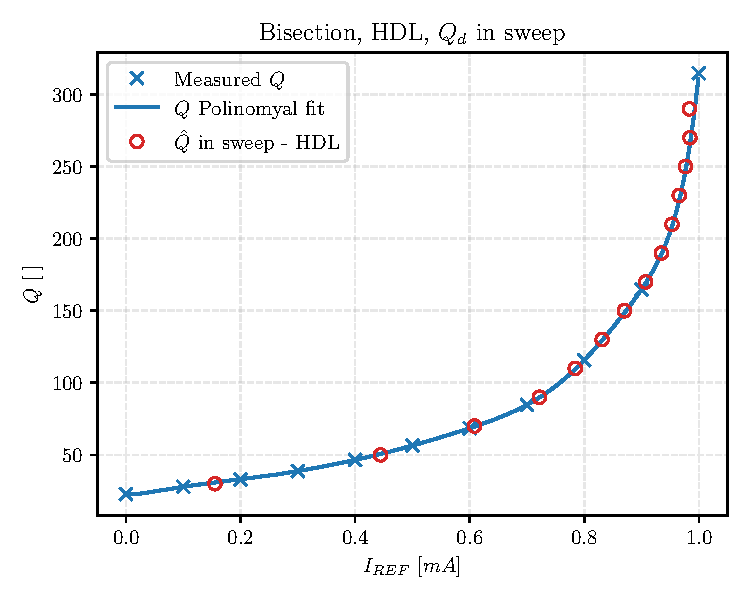
\includegraphics[width=.5\textwidth]{fig/res-bisect-sweep-hdl.pdf}
     \caption*{Fonte: o autor}
    \label{f-sweep-bisect}
\end{figure}
    
\end{frame}


\section{Trabalho futuro}

\begin{frame}[shrink]{Objetivos para o TCC2}

\begin{enumerate}
    \item Codificar módulos restantes em Verilog;
    \item Desenvolver nova codificação para o método das secantes;
    \item Implementar bypass do bloco de controle quando $Q_d \approx Q_{max}$;
    \item Integrar e coordenar a operação dos blocos como um sistema completo;
    \item Selecionar método com melhor desempenho com relação à todo sistema;
    \item Realizar a síntese lógica em RTL;
    \item Simular o circuito sintetizado em RTL e checar a equivalência lógica;
    \item Realizar etapas de posicionamento e roteamento;
    \item Analisar o consumo;
    \item Analisar desempenho do sistema por temporização estática (STA);
    \item Analisar área;
    \item Construir layout.
\end{enumerate}

\end{frame}

\end{document}

